%%%%%%%%%%%%%%%%%%%%%%%%%%%%%%%%%%%%%%%%%
\documentclass[a5paper,doc,10pt,noapacite]{apa6}
%----------------------------------------------------------------------------------------
%	Paquetes y configuraciones
%----------------------------------------------------------------------------------------
\usepackage[hidelinks]{hyperref}
\usepackage[unnumberedbib,notocbib]{apacite}
%\usepackage{chapterbib} % bibunits???
\usepackage{bibunits}

\usepackage{amsfonts} 
\usepackage{amsmath}
\usepackage{amssymb,amsthm}
\usepackage{enumerate}
\usepackage{enumitem}
\usepackage[utf8]{inputenc}
\usepackage[T1]{fontenc}
\usepackage[spanish,es-nolayout,es-nodecimaldot,es-tabla]{babel}
\geometry{top=2.5cm, bottom=2.5cm, left=2.5cm, right=2.5cm, headheight=1.8cm,headsep=.5cm,footskip=1.3cm}

\usepackage{url}
\def\UrlBreaks{\do\/\do-}
\def\pnorm||#1||_#2,#3{||#1||_{L^{#2}(#3)}}
\usepackage{multirow}
\usepackage{multicol}
\usepackage{enumitem}
\usepackage{nicefrac}
\usepackage{graphicx}
\usepackage{stmaryrd}
\usepackage{dsfont}
\usepackage{bropd}
\usepackage{easybmat}
\usepackage[table,xcdraw]{xcolor}
\usepackage{longtable} 
\usepackage{setspace}
\usepackage{comment}
\usepackage{mathpazo}
\usepackage{array}
\usepackage{wrapfig}
\usepackage{ragged2e}
\usepackage{hyperref}
\usepackage{bigstrut}
\usepackage{tabularx}

\usepackage{sectsty}
\sectionfont{\centering\fontsize{13}{15}\selectfont}

\subsectionfont{\centering\fontsize{10}{10}\selectfont\scshape}
\subsectionfont{\fontsize{9.5}{10}\selectfont}

\subsubsectionfont{\centering\fontsize{9}{10}\selectfont}
\paragraphfont{\centering\fontsize{8.5}{10}\selectfont}

\usepackage[titles]{tocloft}
\usepackage{textcomp }

\usepackage{csquotes}
\usepackage{floatrow}

\newfloatcommand{capbtabbox}{table}[][\FBwidth]

% Comandos
\newcommand{\bull}{\textbullet \ }
\newcommand{\EPN}{Escuela Politécnica Nacional}
\newcommand{\Modemat}{Centro de Modelización Matemática, ModeMat-EPN}%{ModeMat -- Escuela Politécnica Nacional}
\newcommand{\Modematb}{Centro de Modelización Matemática, ModeMat-EPN}

\newcommand{\R}{\mathbb{R}}
\newcommand{\N}{\mathbb{N}}
\newcommand{\Z}{\mathbb{Z}}
\newcommand{\C}{\mathbb{C}}
\newcommand{\dsum}{\displaystyle \sum}
\newcommand{\yds}{\qquad\text{y}\qquad}
\newcommand{\tendsto}[1][ ]{\stackrel{ #1 }{\longrightarrow}}
\newcommand{\subKeps}[2][k]{#2_{#1,\varepsilon}}
\DeclareMathOperator{\Dom}{Dom}
\DeclareMathOperator{\Ran}{Ran}
\DeclareMathOperator{\inv}{inv}
\DeclareMathOperator{\Res}{Res}
\DeclareMathOperator{\Ind}{Ind}
\DeclareMathOperator{\im}{Im}
\DeclareMathOperator{\CEiP}{CEiP}
\DeclareMathOperator{\dive}{div}
\DeclareMathOperator{\Esp}{E}
\DeclareMathOperator{\Var}{V}
\DeclareMathOperator{\cov}{cov}
\DeclareMathOperator{\Normal}{\mathcal{N}}
\DeclareMathOperator{\sen}{sen}

\newtheorem{definicion}{Definición}
\newtheorem{proposicion}{Proposición}
\newtheorem{teorema}{Teorema}
\newtheorem{observ}{Observación}
\newtheorem{ejem}{Ejemplo}
\newtheorem*{objetivo}{Objetivo}
\newtheorem*{objetivos}{Objetivos}


%%%mycolors
\definecolor{palegreen}{rgb}{0.6, 0.98, 0.6}
\definecolor{paleblue}{rgb}{0.69, 0.93, 0.93}
\definecolor{pastelyellow}{rgb}{0.99, 0.99, 0.59}
\definecolor{pastelgray}{rgb}{0.81, 0.81, 0.77}
\definecolor{pastelgreen}{rgb}{0.47, 0.87, 0.47}
\definecolor{pastelblue}{rgb}{0.68, 0.78, 0.81}

\newcommand{\vsb}{\vspace{0.75\baselineskip}}
\newcommand{\Speaker}[4]{\vsb #1 \\ \emph{#2} \\ \textsc{#3}\\ \texttt{#4}}


\setlength{\parindent}{0pt}
\linespread{1.5}

\usepackage[10pt]{moresize}

\usepackage{xspace}
\makeatletter
\DeclareRobustCommand{\maybefakesc}[1]{%
  \ifnum\pdfstrcmp{\f@series}{\bfdefault}=\z@
    {\fontsize{\dimexpr0.8\dimexpr\f@size pt\relax}{0}\selectfont\uppercase{#1}}%
  \else
    \textsc{#1}%
  \fi
}
\newcommand\AM{\,\maybefakesc{am}\xspace}
\newcommand\PM{\,\maybefakesc{pm}\xspace}
\makeatother


%---------------------------------------- Autoría ---------------------------------------- %
\title{Plantilla LAWOC}
\author{Andy}
\shorttitle{}
\date{\today}

%---------------------------------------- Citas  ------------------------------------------ %
\renewcommand\bibliographytypesize{\footnotesize}


%------------------------------------- Abstracts ---------------------------------------- %
\newcommand{\pto}{$\cdot$ }

% AbstractA no contiene elementos bibliográficos
\newcommand{\AbstractA}[6]{%
	\addcontentsline{toc}{subsection}{#1 \footnotesize(\emph{#2})}
	\begin{center}
		\bf\scshape#1
	\end{center}
	%\subsection{#1}
	\vspace{-0.85\baselineskip}
	%
	%
	\begin{center}
		{\scriptsize% 
			  #2		\bull			% Autor
		\textsf{#3}		\bull			% Institución
		\texttt{#4}		\\[-1em]		% Correo
		\emph{#5} }				%.Área
	\end{center}
	\vspace{-0.5\baselineskip}
	\begin{spacing}{1.2}
		\footnotesize
		\hspace{15.0pt}
		#6	
	\end{spacing}
	\vspace{1\baselineskip}
}

% AbstractCA no contiene elementos bibliográficos
\newcommand{\AbstractCA}[7]{%
	\addcontentsline{toc}{subsection}{#1 \footnotesize(\emph{#2})}
	\begin{center}
		\bf\scshape#1
	\end{center}
	%\subsection{#1}
	\vspace{-0.85\baselineskip}
	%
	%
	\begin{center}
		{\scriptsize% 
			  #2					% Autor
			  #3		\bull			% Co-autores
		\textsf{#4}		\bull			% Institución
		\texttt{#5}		\\[-1em]		% Correo
		\emph{#6} }				%.Área
	\end{center}
	\vspace{-0.5\baselineskip}
	\begin{spacing}{1.2}
		\footnotesize
		\hspace{15.0pt}
		#7	
	\end{spacing}
	\vspace{1\baselineskip}
}

% Abstract B sí contiene bibliografía
\newcommand{\AbstractB}[6]{%
	\addcontentsline{toc}{subsection}{#1 \footnotesize(\emph{#2})}
	\begin{center}
		\bf\scshape#1
	\end{center}
	%\subsection{#1}
	\vspace{-0.85\baselineskip}
	%
	\begin{center}
		{\scriptsize% 
			  #2		\bull			% Autor
		\textsf{#3}		\bull			% Institución
		\texttt{#4}		\\[-1em]		% Correo
		\emph{#5} }				%.Área
	\end{center}
	\vspace{-0.5\baselineskip}
	\begin{spacing}{1.2}
		\begin{bibunit}
			\footnotesize
			\hspace{15.0pt}
			#6
			\addtocontents{toc}{\protect\setcounter{tocdepth}{-1}}	
			\putbib
			\addtocontents{toc}{\protect\setcounter{tocdepth}{2}}
		\end{bibunit}\vspace{0.5\baselineskip}
	\end{spacing}
}

% Abstract B sí contiene bibliografía
\newcommand{\AbstractCB}[7]{%
	\addcontentsline{toc}{subsection}{#1 \footnotesize(\emph{#2})}
	\begin{center}
		\bf\scshape#1
	\end{center}
	%\subsection{#1}
	\vspace{-0.85\baselineskip}
	%
	\begin{center}
		{\scriptsize% 
			  #2					% Autor
			  #3		\bull			% Co-autores
		\textsf{#4}		\bull			% Institución
		\texttt{#5}		\\[-1em]		% Correo
		\emph{#6} }				%.Área
	\end{center}
	\vspace{-0.5\baselineskip}
	\begin{spacing}{1.2}
		\begin{bibunit}
			\footnotesize
			\hspace{15.0pt}
			#7
			\addtocontents{toc}{\protect\setcounter{tocdepth}{-1}}	
			\putbib
			\addtocontents{toc}{\protect\setcounter{tocdepth}{2}}
		\end{bibunit}\vspace{0.5\baselineskip}
	\end{spacing}
}

% Curso tutorial
\newcommand{\Tutorial}[5]{%
\addcontentsline{toc}{section}{#1 \footnotesize(\emph{#2})}
	\begin{center}
		\bf\scshape #1
	\end{center}
	%\subsection{#1}
	\vspace{-0.85\baselineskip}
	%
	\begin{center}
		{\scriptsize% 
			  #2		\bull			% Autor
		\textsf{#3}		\bull			% Institución
		\texttt{#4}		\\[-1em]		% Correo 
		}
	\end{center}
	\vspace{-0.5\baselineskip}
	%
	
	\begin{spacing}{1}
		\begin{bibunit}
			\footnotesize
			#5
			%\addtocontents{toc}{\protect\setcounter{tocdepth}{-1}}	
			\putbib
			%\addtocontents{toc}{\protect\setcounter{tocdepth}{2}}
		\end{bibunit}\vspace{0.5\baselineskip}
	\end{spacing}
}

%------------------------------------- Información turística ---------------------------------------- %

\newcommand{\InfoTour}[6]{%
\qquad \textbf{\textsc{#1:}}%
#2

\qquad
\begin{tabular}{p{1.5cm} p{7cm}}
	Hours 	& #3
	\\
	Location	& #4
	\\
	Prices	& #5
    \\
    Website & {\scriptsize\texttt{#6}}
\end{tabular}
\vspace{\baselineskip}
}

\newcommand{\InfoTourb}[2]{%
\qquad \textbf{\textsc{#1:}}%
#2
\vspace{\baselineskip}
}

\newcommand{\InfoTourc}[6]{%
\quad \emph{#1:}%
#2

\quad
\begin{tabular}{p{1.5cm} p{7cm}}
	Hours 	& #3
	\\
	Location	& #4
	\\
	Prices	& #5
    \\
    Website & {\scriptsize\texttt{#6}}
\end{tabular}
\vspace{\baselineskip}
}

\newcommand{\Rest}[3]{%
\begin{tabular}{>{\bf\scshape}p{3.5cm} >{\em\centering\arraybackslash}p{2cm}    >
{\raggedleft\arraybackslash}p{4cm}}
	#1  & #2 & #3
\end{tabular}
\vspace{0.4\baselineskip}
}

\renewcommand{\BCBT}{}

% -------------- Pseudo definición fuera de entorno que no me gustó pero toca respetar las malas costumbres de algún modo

\newcommand{\neodefi}[1]{%
	\vspace{1\baselineskip}
	\textbf{\small#1} \newline
}

%--------------------------------------------------------------------------------------------------------------------------------------
%----------------------------------------------------------------------------------------
%------------------------------------------
\begin{document}
\pagestyle{empty}
\pagenumbering{gobble} 
%%%%%%%%%%%%%%%%%%%%%%%%
%      Título
%%%%%%%%%%%%%%%%%%%%%%%%
\newgeometry{top=4cm, bottom=2cm, left=2.5cm, right=2.5cm}
{
	\HUGE
	{\bf\textsc{XVI \\[0.5cm] Encuentro  \\[0.5cm] de Matemática \\[0.5cm] y sus Aplicaciones \\[0.5cm] }}
	\\[1cm]
	\large
	
	\vspace{-2.cm}
	\begin{center}
		
		\textsc{El Arte de hacer Estadísticas: Estadística básica para personas con alma de artista. ¡Desarrolla tu propia encuesta online!}
		
		\vspace{1.25\baselineskip}
		
		Gabriela Castro
		\\
		
		\normalsize
		Sociedad Ecuatoriana de Estadística, Ecuador
	\end{center}

}

\vspace{1.5cm}
\begin{center}
	
\includegraphics[height=2.45cm]{Logos/DM-EPN}
\end{center}

%\clearpage\null\newpage
%%%%%%%%%%%%%%%%%%%%%%%%
%      Datos de edición
%%%%%%%%%%%%%%%%%%%%%%%%
\newpage
\newgeometry{top=4cm, bottom=2cm, left=2cm, right=2cm}
\mbox{}
\vfill
{
\footnotesize
\textsc{XVI Encuentro de Matemática y sus Aplicaciones}

22 -- 26 de octubre de 2018

Quito, Ecuador

%
\vspace{1\baselineskip}
\emph{Comité Organizador}
\begin{spacing}{1.2}
\scriptsize
	Polo Vacas		\bull Paúl Acevedo	\bull Adriana Uquillas	
	
	\emph{\EPN}
\end{spacing}

%
\vspace{1\baselineskip}
\emph{Comité Científico}
\begin{spacing}{1.2}
\scriptsize
	Marco Calahorrano Recalde	--	\emph{\EPN, ECUADOR} 		\bull 
	Diego Chamorro			-- 	\emph{Université d'Évry, FRANCIA} \bull
	Juan Carlos De los Reyes		-- 	\emph{\EPN, ECUADOR} \bull
	Luis Horna				--	\emph{\EPN, ECUADOR} \bull
	Luis Miguel Torres			--	\emph{\EPN, ECUADOR} 
%		
\end{spacing}

%
\vspace{1\baselineskip}
\emph{De esta edición}
\begin{spacing}{1.2}
\scriptsize
	\emph{Editor:} 	Andrés Miniguano Trujillo 	--	\emph{\Modemat, ECUADOR}
	
	\emph{Asistentes:} Eduardo Arias, Erika Ludeña -- \emph{\EPN, ECUADOR}
	
	\emph{Diseño arte:} Julio Erazo -- \emph{\EPN, ECUADOR}
	
	\emph{Adaptación de portada:} Belén Santacruz Reyes
%		
\end{spacing}

%
\vspace{1\baselineskip}
\emph{Auspiciantes}
\begin{spacing}{1.2}
\scriptsize
	Sociedad Ecuatoriana de Matemática \emph{(SEdeM)}				\bull
	\Modemat													\bull
	Actuaria: Asesoramiento Estratégico
\end{spacing}

%
\vspace{1\baselineskip}
\emph{Con el apoyo de}
\begin{spacing}{1.2}
\scriptsize
	Escuela Politécnica Nacional \emph{(EPN)}						\bull
	Departamento de Matemática EPN
\end{spacing}


% Logos
\vspace{1.5\baselineskip}
\begin{center}
	
\includegraphics[height=1cm]{Logos/SEdeM}
	\qquad\quad
	
\includegraphics[height=1cm]{Logos/ModeMat}
	\qquad\quad
	
\includegraphics[width=2.5cm]{Logos/logo-actuaria}			%*
	\qquad\quad
	
\includegraphics[height=1cm]{Logos/EPN}
	\qquad\quad
	
\includegraphics[height=1cm]{Logos/DM-EPN}
\end{center}

% Contenidos
\newpage
\pagestyle{empty}
\pagenumbering{arabic}
\setcounter{page}{0}
\newgeometry{top=2cm, bottom=2cm, left=2cm, right=2cm, headheight=1.8cm,headsep=.5cm,footskip=1.3cm}
%\normalsize
\small
\tableofcontents



%----------------------------------------------------------------------------------------
\newpage
\pagestyle{plain}
%%%%%%%%%%%%%%%%%%%%%%%%
%%%%%%%%%%%%%%%%%%%%%%%%
% \section{Program}
% \normalsize
% adad
%que no pongamos el programa


%----------------------------------------------------------------------------------------
\newpage
%%%%%%%%%%%%%%%%%%%%%%%%
%%%%%%%%%%%%%%%%%%%%%%%%
\newgeometry{top=2cm, bottom=2cm, left=1.75cm, right=1.75cm, headheight=1.8cm,headsep=.5cm,footskip=1.3cm}

\begin{comment}
\section{Presentación}
\footnotesize

The VI Latin American Workshop on Optimization and Control will take place in Quito, Ecuador, September 3 - 7, 2018. The event is organized on a biennial basis with the main goal of boosting the development and interaction between these two scientific disciplines in Latin America. Therefore, the workshop gathers outstanding senior and junior researchers, postdoctoral fellows, and graduate students working in these fields.

\vspace{0.5\baselineskip}
The event focuses, among others, on the following topics:
\begin{APAitemize}
	\item Optimal Control
    \item Inverse Problems
    \item Nonsmooth Optimization
    \item Control of Partial Differential Equations
\end{APAitemize}

\vspace{0.5\baselineskip}
The first edition of this event was held in Quito, Ecuador, in July 2008, based on an initiative of researchers from Escuela Politécnica Nacional, Ecuador, and Universidad Nacional de Rosario, Argentina. The second edition was held in 2010 in Rosario, Argentina, with the same organizers. Subsequently, a third edition took place in 2012 in Valparaiso, Chile; a fourth edition in 2014 in Lima, Peru; and a fifth edition was held in 2016 in Tandil, Argentina.

\vspace{0.5\baselineskip}
An additional goal of the workshop is to increase of visibility of Optimization and Control among advanced undergraduate students (in Mathematics, Computer Science, Engineering, Physics, Economics and others).
\end{comment}

%----------------------------------------------------------------------------------------
\newpage
%%%%%%%%%%%%%%%%%%%%%%%%
%%%%%%%%%%%%%%%%%%%%%%%%
\newgeometry{top=2cm, bottom=2cm, left=1.75cm, right=1.75cm, headheight=1.8cm,headsep=.5cm,footskip=1.3cm}

\bibliographyunit[\subsection]
\bibliography*{citas.bib}
\bibliographystyle*{apacite}
\bibliographyunit
\renewcommand{\refname}{\small Referencias}



%----------------------------------------------------------------------------------------


%%%%%%%%%%%%%%%%%%%%%%%%
%%%%%%%%%%%%%%%%%%%%%%%%
%
\footnotesize
\normalsize



% ------------------ Castro ------------------%
\Tutorial{El Arte de hacer Estadísticas: Estadística básica para personas con alma de artista. ¡Desarrolla tu propia encuesta online!}{Gabriela Castro}{Sociedad Ecuatoriana de Estadística, Ecuador}{gaby77castro@gmail.com}{
	\subsection{Orígenes de la estadística}

Se puede considerar dos de las actividades que han realizado los seres humanos, como las bases para los orígenes de la estadística, son las siguientes:

\vspace{1\baselineskip}
\textbf{El interés por registrar todo lo que le rodea:} Los seres humanos siempre han estado atentos a su entorno y han buscado registrar lo que está a su alrededor, mediante pinturas rupestres en cuevas, esculpe sobre huesos, madera, tablas de arcilla papiros o papel \cite{Fernandez-2002}.

Los primeros registros se relacionan a actividades de caza, religiosas o guerras; pero a medida que aparecen la primera civilización los registros se convierten en una herramienta necesaria para los Estados, que buscan contar con registros de propiedades, censos de población, transacciones
económicas, disponibilidad de recursos \cite{Fernandez-2002}.

La segunda se relaciona con la \textbf{afición de los seres humanos por los juegos de azar}; esta es una afición surgida desde los comienzos de la humanidad, según se ha encontrado en yacimientos arqueológicos muy antiguos. Esta afición exige buscar la solución más favorable para sus
intereses; es decir, la solución que de brinde mayor probabilidad de éxito \cite{Fernandez-2002}.

\subsubsection{Un poco de historia de la Estadística en Ecuador.}

En la \textbf{época incásica} el Tahuantinsuyo habitaba una población estimada en más de 12 millones de personas, que se agrupaban en una multiplicidad de etnias diferente; que, aunque compartían algunos atributos culturales, diferían en otros aspectos como el lenguaje, lo que representaba un problema para el compartir de ideas, tales como la programación de las actividades burocráticas, la administración de los bienes y actividades estatales repartidas por todo el Imperio. 

\begin{wrapfigure}{l}{0.25\textwidth} %this figure will be at the right
    \centering
    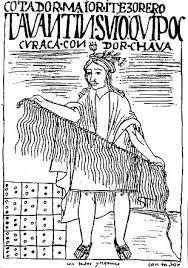
\includegraphics[scale=0.35]{Graficos/fig5_GC.jpg}
\end{wrapfigure}

En este sentido, una de las herramientas más importantes fueron los \textbf{quipus}, proveniente del vocablo quechua que significa <<nudo>> ; se refiere a un implemento de cuerdas anudadas que fue el principal instrumento para registrar información en el Imperio Inca.

A partir de la conquista, los españoles relatan que la información contenida en los quipus incluía datos estadísticos relacionados con el registro de censos, la contabilidad tributaria y otras informaciones numéricas similares. 

\begin{wrapfigure}{r}{0.25\textwidth} %this figure will be at the right
    \centering
    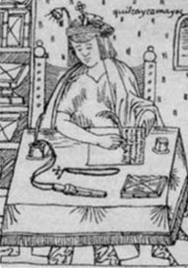
\includegraphics[scale=0.35]{Graficos/fig3_GC.jpg}
    \vspace{-2em}
\end{wrapfigure}

En la \textbf{época colonia}, en las últimas décadas del siglo XVIII, comenzó un proceso de recolección de información que la Corona española requería de sus posesiones americanas. Es así que los ministros en cada uno de sus ramos respectivos, comenzaron a utilizar la frase \textquote{Su majestad quiere saber}, a fin de recabar toda esa información necesaria para planificar correctamente un futuro de seguridad y promisión para los territorios americanos. A fines del siglo XVII, se comenzó a utilizar la frase: \textquote{Su Majestad quiere una exposición clara y sencilla}.

\vspace{1\baselineskip}
La cantidad de información almacenada sin revisar y su escasa utilización dieron muestra del poco interés que demostraron los políticos y funcionarios de esa época, y es solo a finales del siglo XX cuando se comienza a valorar este bagaje de información.

\begin{wrapfigure}{l}{0.35\textwidth} %this figure will be at the right
    \centering
    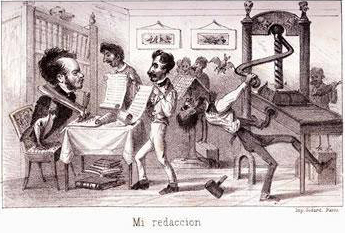
\includegraphics[scale=0.3]{Graficos/fig1_GC.jpg}
\end{wrapfigure}

Durante la \textbf{época republicana}, se hicieron intentos de institucionalizar la ejecución de de censos a través de la expedición de leyes o decretos que permitieran su realización, normas legales que se han perdido o se encuentran dispersas entre gran cantidad de archivos históricos de nuestro país. 

\vspace{1\baselineskip}
Así, por ejemplo, en la Primera Constitución del Estado del Ecuador de 1830, al disponerse que la representación de diputados de los tres departamentos (Azuay, Guayas y Quito) que conformaron el <<Estado del Ecuador>>, se la haría según el censo de población; en 1873 el presidente García Moreno decretó la creación de una Oficina de Estadística, en la ciudad de Quito; durante la presidencia de Velasco Ibarra, en 1970, se decreta que las funciones de Estadísticas y Censos serán ejercidas a través del Instituto Nacional de Estadísticas (INE). Finalmente, en 1976 y en 1978, se expide la Ley de Estadística, vigente hasta esta fecha, en la que se crean el Sistema Estadístico Nacional (SEN), el Consejo Nacional de Estadística y Censos (CONEC) y el Instituto Nacional de Estadística y Censos (INEC).

\vspace{1\baselineskip}
En la \textbf{actualidad}, esta ciencia es tiene gran aplicabilidad, hasta el punto de no concebir un trabajo de carácter científico sin el apoyo de algún método estadístico. 

\begin{wrapfigure}{r}{0.25\textwidth} %this figure will be at the right
    \centering
    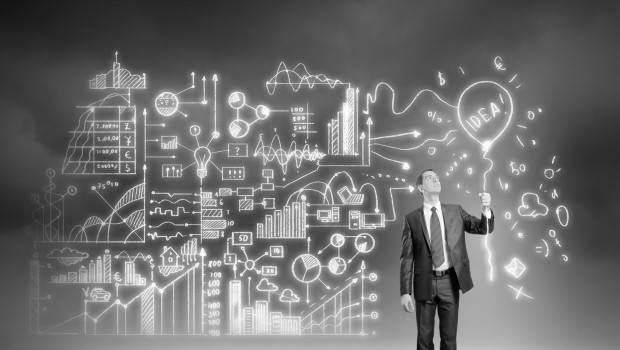
\includegraphics[scale=0.12]{Graficos/fig9_GC.jpg}
    \vspace{-1em}
\end{wrapfigure}

Se ha convertido en un elemento fundamental de la sociedad de la información y del conocimiento, en la cual se desarrolla el mundo y el Ecuador.

El Ecuador se ha avanzado en cuanto a la generación de información estadística, se cuenta con un Instituto Nacional de Estadística más fortalecido; así como el Banco Central de Ecuador, encargado de la generación de las estadísticas de síntesis de los principales sectores de la economía; el país cuenta con el Sistema Nacional de Información a cargo de la Secretaría Nacional de Planificación y Desarrollo. Sin embargo, es innegable que en nuestro medio existe un vacío notorio en lo referente a la evolución de la estadística, debido a falta de obras que recojan y organicen la información dispersa y proporcionen una amplia y selecta bibliografía como fuente de consulta.

\vspace{1\baselineskip}
En el país existen diversas situaciones que impiden el desarrollo de las actividades estadísticas, a la par de las tendencias de los países más desarrollados, tales como: escaso financiamiento, la falta consciencia por parte de los gobernantes sobre la importancia de la estadística para la toma de decisiones, la falta de cultura estadística nacional de productores, informantes y usuarios, la limitada armonización e integración de la información, la falta de decisión política y la falta de capacitación del personal involucrado el trabajo estadístico.

\newpage
\subsection{¿Qué es la Estadística?} 

La estadística es una ciencia teórica que forma parte de las ciencias matemáticas; facilita la toma de decisiones mediante la presentación ordenada de los datos a través de tablas y gráficos estadísticos; también permite reducir los datos observados a un pequeño número de medidas estadísticas que permitan la comparación entre diferentes series de datos; además, permite estimar la probabilidad de éxito que tiene cada una de las decisiones posibles \cite{Fernandez-2002}.

\subsubsection{Ramas de la estadística}

La estadística se puede dividir en dos ramas principales, la estadística descriptiva y la estadística analítica:

\vspace{1\baselineskip}
La \textbf{estadística descriptiva} tiene como objeto representar y resumir los resultados, \([...]\) En general se condensa la información obtenida, en tablas, gráficos y parámetros que la resumen y permiten entenderla rápidamente \cite{Vargas-1995}. <<La reducción de datos conlleva a un error que debe ser controlado, puede realizarse previamente durante el proceso de tabulación o, con mayor eficacia, utilizando las medidas estadísticas>> \cite{Fernandez-2002}, las mismas que permitirán comparar diferentes series de datos obtenidas mediante diversas observaciones.

La \textbf{estadística analítica}, también denomina inferencial, estudia los elementos de una muestra y a través de la construcción de un modelo matemático infiere las propiedades a la población muestreada. Estudia la probabilidad de éxito de diferentes soluciones posibles a un problema de las diferentes ramas de la ciencia.

\subsection{Conceptos básicos de la estadística}

\textbf{Población:} Cualquier conjunto de personas, objetos, ideas, o acontecimientos que se someten a una observación estadística de una o varias características que comparten sus elementos y que permiten diferenciarlos. El significado de población en la estadística es más amplio que el utilizado en el lenguaje común, que suele hacer alusión al conjunto de personas.

\textbf{Elementos o individuos de una población:} son cada uno de los componentes de la población.

\textbf{Tamaño de la población:} es el número de elementos de una población, que puede ser finito o infinito.

\textbf{Caracteres de una población:} son cada una de las propiedades, rasgos, o cualidades que poseen los elementos de una población.

\textbf{Variable:} es cualquier carácter de una población susceptible de tomar valores numéricos; en todos los elementos de una población no se presenta la misma intensidad de cada uno de dichos valores.

Las variables se clasifican en continuas y discretas, según admitan o no infinitos valores intermedios entre dos valores próximos respectivamente.

\textbf{Muestra:} es la parte seleccionada de una población, en la que los elementos que son parte, no tiene ninguna característica esencial que los distinga del resto. Se utiliza cuando se pretenden contar con una parte representativa de la población.

\textbf{Censos:} son observaciones exhaustivas que estudias los caracteres estructurales y estáticos de toda una población.

\textbf{Encuestas:} son investigaciones realizadas sobre un subconjunto de la población, generalmente son realizadas sobre fenómenos más dinámicos de la población; los datos se obtienen. 

\textbf{Frecuencia:} es el número de repeticiones que presenta un determinado dato de un carácter en los diferentes elementos de una población o muestra.

\textbf{Frecuencia absoluta:} es el número de repeticiones de un determinado valor de una variable. También representa el número de elementos de la población que tiene el mismo valor o modalidad. La suma de frecuencias corresponde al tamaño de la población.

\textbf{Frecuencia relativa:} es una proporción entre el número de veces que se repite un dato y el tamaño de la población. Se obtiene de dividir la frecuencia absoluta de un determinado dato entre el tamaño de la población.  

\subsection{Tipos de medidas de los datos}

\textbf{Medida Nominal (datos categóricos):} se refiere a caracteres cualitativos o atributos, no tienen ninguna relación de orden, no puede medirse en una escala continua. Por ejemplo, los colores de cabellos, sexo, sabores de helados, etc.

\textbf{Medida ordinal (datos de tipo ordinal):} en este caso son caracteres cualitativos, pero que tienen una relación de orden; no puede fijarse una distancia entre dos datos consecutivos. Por ejemplo, los niveles educativos, las categorías laborales de una empresa.

\textbf{Medidas cuantitativas o de intervalo:} los datos tienen un orden, es posible medir la distancia entre dos valores cualquiera, pueden ser variables descritas, como número enteros o continuas cuando hay infinitos número en sus intervalos. Por ejemplo, la temperatura, la edad, el salario,
el peso corporal.

\subsection{Medidas de posición}

Las medidas de posición representan puntos de referencia que permiten ubicar la situación de una variable estadística en la recta real y de este modo mostrar la síntesis de toda la información contenida en la distribución de frecuencias.

\textbf{Moda:} identifica el valor o intervalo que más se repite, es el valor que se ha observado un mayor número de veces (Casares. 2007).

Se debe tener precaución con el valor modal, puesto que puede ser engañoso, ya que no necesariamente indica la ubicación de la mayoría de los valores de la distribución en su conjunto (Casares. 2007).

\textbf{Medidas de tendencia central}

Las medidas de tendencia central muestran la localización o posición de los valores alrededor de los cuales fluctúan los demás \cite{Vargas-1995}.

\textbf{Media o promedio} se define como la división entre la suma de los valores que toma una variable respecto al total de elementos de una muestra. Se representa con el símbolo , se calcula con la siguiente fórmula \cite{Vargas-1995}:   
\[
	\bar{x}= \dfrac{1}{n} \sum \limits_{i=1}^{n} x_{i} = \dfrac{x_{1}+x_{2}+ \cdots+x_{n}}{n}
\]

Donde:
\begin{APAitemize}
\item \(\bar{x}\): es el valor promedio de la variable.
\item \(x_{i}\): son los valores que toma el elemento \(i\) de la variable.
\item \(n\): es el total de elementos de una muestra.
\item \(\sum\): es la sumatoria.
\end{APAitemize}

\vspace{1\baselineskip}
\textbf{Mediana:} es el dato que se encuentran en el lugar central de un conjunto de datos ordenados. 



\newpage



\subsection{Medidas de dispersión}
Las medidas de dispersión permiten evidenciar que tan alejados se encuentran los datos de la media.

\vspace{1\baselineskip}
\textbf{Desviación media:} Es la división entre la suma de los valores absolutos de las diferencias entre cada uno de los valores y el promedio respecto al total.
\[
	D_{m}= \sum_{i=1}^{n} \dfrac{|x_{i} \cdot \bar{x}|}{n}
\] 

\textbf{Varianza muestral:} es el promedio de las diferencias cuadráticas de los datos respecto al promedio; y sus unidades son las unidades de los datos al cuadrado. Su fórmula es la siguiente \cite{Vargas-1995}:
\[
	S^{2}= \sum_{i=1}^{n} \dfrac{ \left( x_{i}-\bar{x} \right)^{2}}{n-1}
\]

\textbf{Desviación estándar:} es la raíz cuadrada de la varianza. Las unidades de medida de la desviación típica son las mimas que la de los datos sobre los que ha sido calculada.
\[
	S= \sqrt{ \sum_{i=1}^{n} \dfrac{ \left( x_{i}-\bar{x} \right)^{2}}{n-1} }
\]


\subsection{Representaciones gráficas}

Un gráfico proporciona una impresión que ayuda a clasificar la variabilidad y simetría de los datos. Existen diferentes tipos de gráficos que dependen de la naturaleza del tipo de la variable que se esté analizando.

\begin{table}[H]
\fontsize{7}{11}\selectfont
  \centering
    \begin{tabular}{c | p{9em} | c} \thickline
    	\textbf{Tipo de variable} & \textbf{Gráfico} & \textbf{Representación} \bigstrut\\ \hline
    	Cualitativa & Diagrama de rectángulos o Barras & \raisebox{-\totalheight}{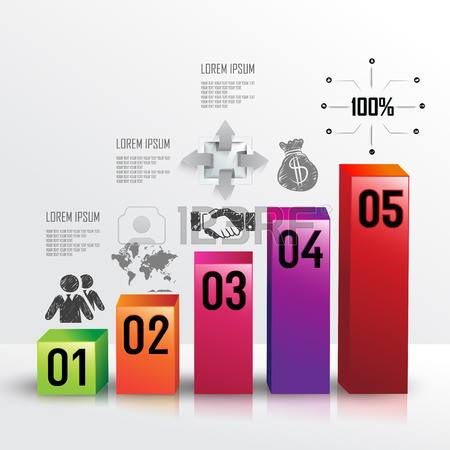
\includegraphics[width=3cm]{Graficos/fig2_GC.jpg}} \\
        & Sectores o pasteles &  \raisebox{-\totalheight}{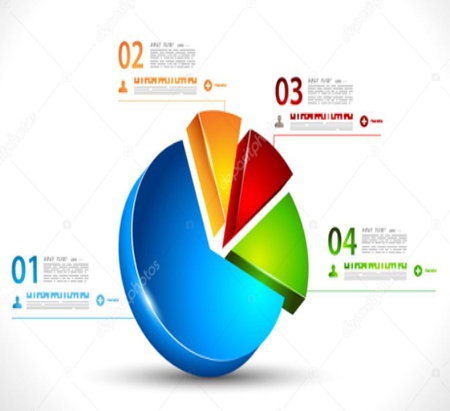
\includegraphics[width=3cm]{Graficos/fig11_GC.jpg}} \\
    \thickline
    \end{tabular}
\end{table}

\begin{table}[H]
\fontsize{7}{11}\selectfont
  \centering
    \begin{tabular}{c | p{9em} | c} \thickline
    \multicolumn{1}{p{7.5em}|}{} & Pictogramas & \raisebox{-\totalheight}{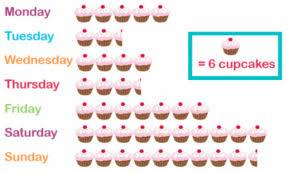
\includegraphics[width=3cm]{Graficos/fig7_GC.jpg}} \\          
          & Perfil radial & \raisebox{-\totalheight}{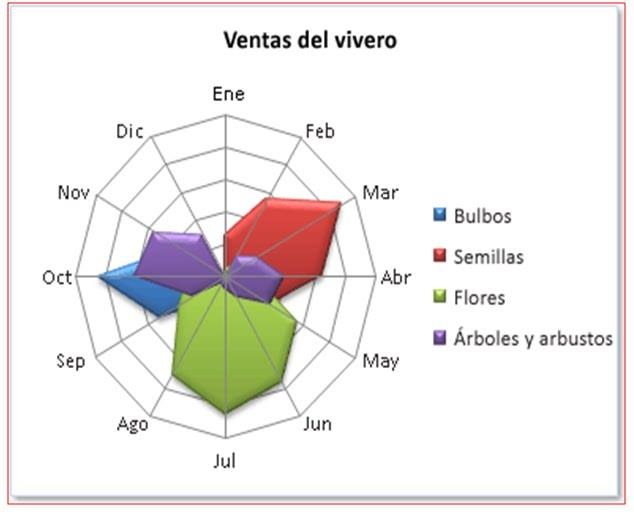
\includegraphics[width=3cm]{Graficos/fig10_GC.jpg}} \\
          & Cartograma & \raisebox{-\totalheight}{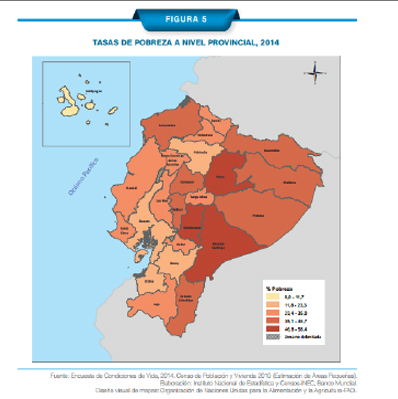
\includegraphics[width=3cm]{Graficos/fig12_GC.jpg}} \\
    \thickline
    \end{tabular}
    \end{table}
    
\begin{table}[H]
\fontsize{7}{11}\selectfont
  \centering
    \begin{tabular}{c | p{9em} | c} \thickline
    \textbf{Tipo de variable} & \textbf{Gráfico} & \textbf{Representación} \bigstrut\\ \hline
    {Cuantitativa} & Histograma & \raisebox{-\totalheight}{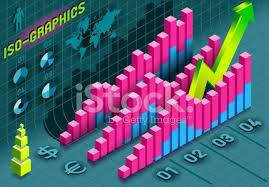
\includegraphics[width=3cm]{Graficos/fig6_GC.jpg}} \\
	& Polígono de \newline frecuencias simples &  \raisebox{-\totalheight}{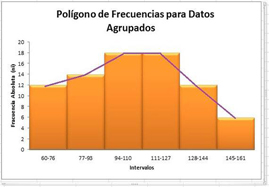
\includegraphics[width=3cm]{Graficos/fig8_GC.jpg}}\\
    & Diagrama de\newline frecuencias acumuladas \newline Variables discretas &  \raisebox{-\totalheight}{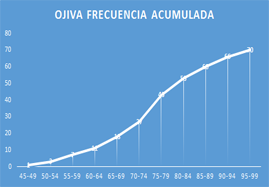
\includegraphics[width=3cm]{Graficos/fig31_GC.png}} \\
    \thickline
    \end{tabular}
\end{table}




\subsection{¿Cómo hacer una encuesta?}

La gran mayoría de oficinas de estadística del mundo se rigen por el modelo de producción estadística para la generación de operaciones estadísticas, que <<se define como el conjunto de actividades que involucran, de acuerdo a su naturaleza, la ejecución de las fases y procesos del Modelo Genérico de Producción Estadística. Los procesos incluyen la planificación, diseño, construcción, recolección, procesamiento, análisis, difusión y evaluación de los resultados estadísticos sobre determinada área o tema de interés nacional>> (IENC, 2014). Las encuestas, censos, estadísticas con base en registros administrativos son operaciones estadísticas.

El modelo de producción estadística es un proceso que determina las fases que se deben seguir para implementar una operación estadística. El modelo está diseñado para ser implementado independientemente del tipo de fuente de datos utilizada para la generación de estadísticas. Para Ecuador, este modelo fue desarrollado por el Instituto Nacional de Estadística y Censos; consta de ocho fases y dos macro procesos transversales.

Se presenta a continuación, de manera sucinta las ocho fases del Modelo de Producción Estadística y las actividades que conllevan cada una de ellas.

\begin{figure}[H]
	\fontsize{7}{11}\selectfont
	\captionsetup{justification=centering, labelfont=footnotesize, font=footnotesize}
\caption*{Modelo de producción estadística}
\centering
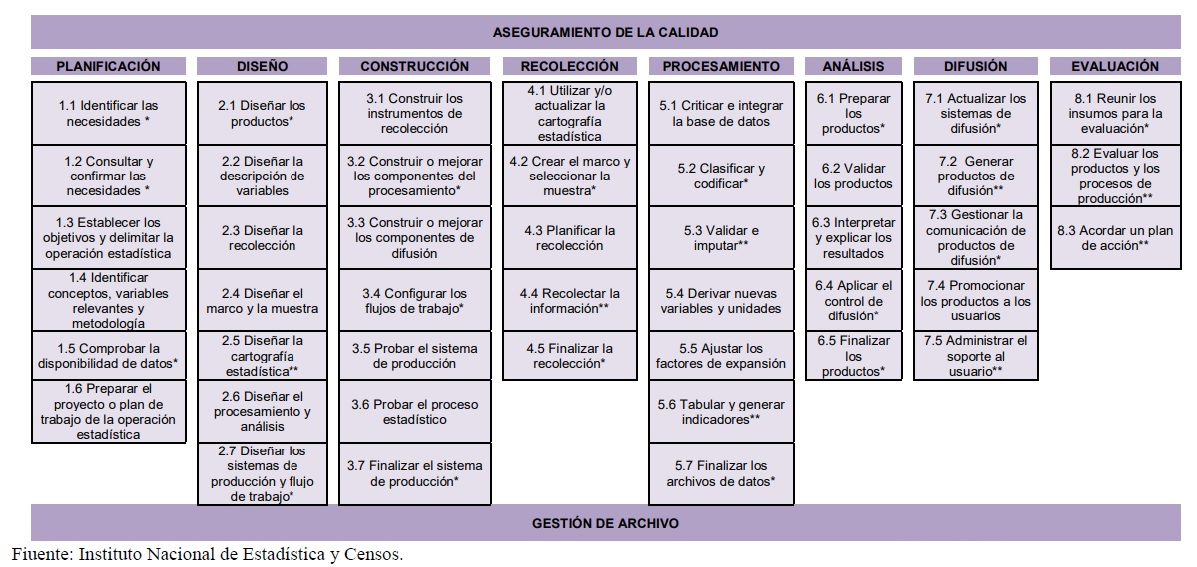
\includegraphics[scale=0.35]{Graficos/fig14_GC.jpg}
\end{figure}

\subsection{Desarrollo de encuestas en línea}
En la actualidad el mundo está cada vez más sumido en la tecnología, el uso de los dispositivos tecnológicos es cada vez más común y se usa sin diferencia de edad o estrato social. La sociedad, cada vez más, está automatizando todas las actividades que se realizan a diario, sea a la hora de estudiar, trabajar, o actividades cotidianas.

En este sentido las técnicas para recabar datos se están volcando a la utilización de herramientas tecnológicas, como los dispositivos móviles (tablet, laptop, celulares) y los computadores; otorgando a cada persona que las usa, una rapidez mayor. En tal sentido, se han convertido en una forma, cada vez más utilizada, para levantar información. Aunque cabe destacar que los procesos presenciales para recopilar información no han dejado de estar vigentes.

Este tipo de herramientas son comúnmente utilizadas en el marketing digital, estudios de mercado, puesto que las empresas consideran que las encuestas online son un medio adecuado para evaluar los niveles de satisfacción mediante la web. Por ejemplo, a través de encuestas se evalúan los productos que los consumidores creen mejor que otros o la calidad de los mismos y a partir de dicha información los analistas tiene elementos paras crear estrategias que puedan ser de beneficio para una institución.


	\begin{center}
	\fontsize{7}{11}\selectfont
	\begin{tabularx}{\textwidth}{X X}
		\thickline
		\textbf{Ventajas} & \textbf{Desventajas} \\	\hline
Son económicas, existe mucho ahorro en contratación de encuestadores, desarrolladores de aplicativos para la recolección de datos, entre otros. & Puede existir desconfianza del encuestado, lo que promovería que las respuestas no sean totalmente ciertas. \\
Se obtienen resultados de manera más rápida, al tener automatizado el ingreso de los datos a través de las aplicaciones web. & Sesgo en los resultados, es decir, análisis que se realice, no se podrá inferir sobre el total del universo, ya que no se puede conocer qué porcentaje representa la muestra y si este es suficiente, como para ser considerado.\\
    Aportan valor, porque al hacer una encuesta a los clientes, por ejemplo, al terminar un proceso de compra, demuestra la preocupación por el trabajo bien hecho. & Baja fiabilidad estadística, al no tener un universo conocido y una muestra representativa, los indicadores estadísticos no siempre funcionan con el nivel de fiabilidad requeridos. \\
		\thickline
		\\[3em]
	\end{tabularx}
	\label{tab:B1}

	\emph{Ventajas y desventajas de las encuestas Online}
	\end{center}


\textbf{Nota importante:} Si se quiere usar una encuesta online, generando datos cuantitativos, es necesario respetar y analizar los porcentajes que se obtienen, como porcentajes sobre el total de respuestas, no sobre la población que se está estudiando.

\vspace{1\baselineskip}
Hoy en día existen varias herramientas web a través de las cuales se pueden elaborar encuestas en línea, tales como:

\vspace{1\baselineskip}
\textbf{Google.}
La empresa de google tiene el servicio de encuestas por medio de sus productos de google drive, que permite, de manera gratuita, crear formularios de encuestas, mostrando diferentes plantillas o se crear una propia. Esta herramienta permite analizar los datos luego de ser obtenidos, al crear una base de datos con la información se va recopilando.

\textbf{TypeForm.}
Es un sitio web que ofrece la vista adecuada para las encuestas, el principal interés es que el usuario no abandone el proceso de la encuesta ya sea por las aburridas preguntas o una vista que no le agrada; busca que el internauta observe la encuesta sin importar las preguntas.

\textbf{Survio.}
Es una herramienta bastante popular, que cuenta con un repertorio de 100 platillas o más para emplear. Tiene las opciones de compartir en las redes sociales y ofrece características para evaluar el mercado de comercio entre las empresa.

\textbf{Polldady.}
Es una herramienta que permite crear encuestas on line con la ayuda de un editor visual, de arrastrar y soltar, destaca por la elegancia de sus estilos visuales, las matrices de preguntas y la posibilidad de trabajar con contenido multimedia propio.

\vspace{1\baselineskip}
En este documento nos centraremos en el desarrollo de encuestas con Google Drive, sus ventajas son:

\begin{APAitemize}
\item Costo <<cero>>, por ser gratuito.
\item Se puede obtener respuestas, visualizar estadísticas y obtener resultados a tiempo real.
\item Permite organizar los formularios de manera totalmente personalizada: con logotipo de la empresa, añadiendo imágenes, vídeos, podcast. 
\item Es muy poco intrusivo. La persona encuestada puede elegir contestar cuando lo desee.
\item Se puede segmentar; esto es, si se cuenta con una base de datos, es posible enviar diferentes tipos de encuestas según la edad, sexo, localización, poder adquisitivo.  
\item Las encuestas se recopilan automáticamente generando estadísticas para facilitar la obtención de resultados y su posterior análisis.
\item Los encuestados pueden responder de manera instantánea ya sea desde el ordenador, móvil o tablet.  
\end{APAitemize}

\subsubsection{Desarrollo de un formulario Online en Google Drive.}

Para el desarrollo de un formulario online se siguen los siguientes pasos:

\begin{APAenumerate}
\item Acceder a una cuenta de Google. 
\item Ir a la opción Google drive y seleccionar el apartado de formularios. 
\item Diseñar la encuesta.

\subitem Poner el título de la encuesta 
\subitem Se debe elegir el tipo de pregunta que se requiere hacer; estas pueden ser: de texto, respuesta única, respuesta múltiple, selección de una opción de una lista.
\subitem Luego se poner <<Agregar elemento>> y se continúa añadiendo preguntas. 
\subitem En la barra superior del área de trabajo dar click en <<Ver el formulario publicado>> para ver cómo está quedando el formulario.

\item Una vez terminado dar click en <<Enviar formulario>> y se abrirá una nueva ventana con diversas opciones para distribuir el formulario, sea este mediante redes sociales, correo electrónico, vincularlo a un sitio web. 
\end{APAenumerate}

\subsection{Visualización de la información}
En este mundo cambiante, lleno de imágenes, es importante la forma en la que la información se presenta. Es por esto, que se han desarrollado varias herramientas online para crear infografías que permitan mostrar los resultados de una manera más atractiva al público en general, y que sea más fácil de comprender y digerir.

Entre los sitios web más conocidos para la creación de infografías se tiene:

\vspace{1\baselineskip}
\textbf{Canva.}
La herramienta de creación de infografías en Canva contiene cientos de elementos de diseño  gratuitos, lo que permite experimentar con la visualización de datos con mucha versatilidad.

\textbf{Info.gram.}
Es una herramienta gratuita que permite insertar información en cada una de las cajas predeterminadas, se puede añadir y eliminar cajas. Se puede elegir más de una docena de opciones gráficas, añadir cajas de texto, fotos, mapas o incluso videos. Es posible compartir la infografía en redes sociales o usar el código para ponerla en un sitio Web.

\textbf{Google Developers.}
Esta es una herramienta de Google, fácil de utilizar y además gratuita. Se puede elegir entre una amplia variedad de gráficos y, que permite conectarlos con los datos generados en tiempo real por una web.

\textbf{Piktochart.}
El editor de Piktochart permite modificar el color de las fuentes, insertar gráficos y cargar formas e imágenes. Es sencillo alinear los diferentes elementos gráficos que integran la infografía y modificar el tamaño de las imágenes de manera proporcional.

\vspace{1\baselineskip}
\textbf{Ejemplo de una infografía:}

\begin{figure}[H]
\fontsize{7}{11}\selectfont
\captionsetup{justification=centering, labelfont=footnotesize, font=footnotesize}
\centering
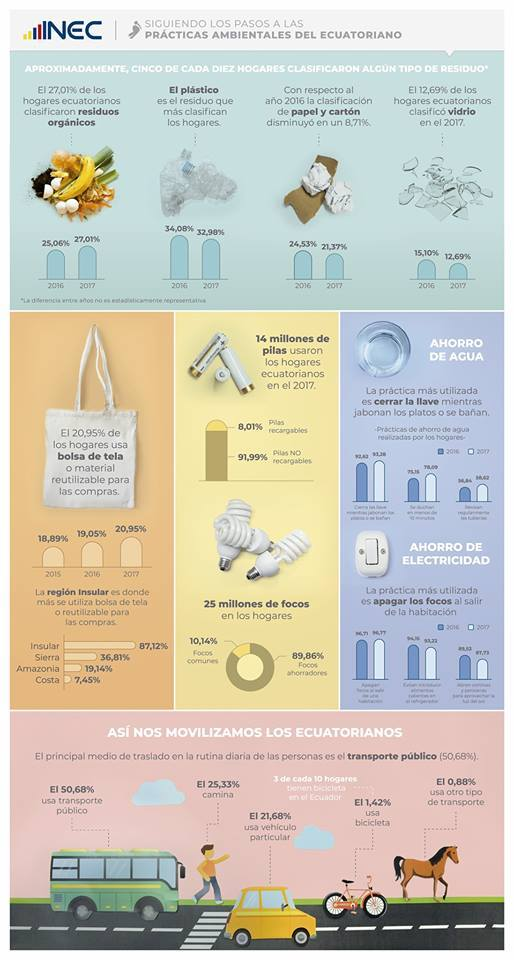
\includegraphics[scale=0.39]{Graficos/fig4_GC.jpg}
\caption*{Fuente: Instituto Nacional de Estadística y Censos}
\end{figure}

\newpage

\nocite{Caceres-2007, Arribas-2014, CaceresH-2007, INEC-2014, Ross-2007}
}








\end{document}































